\documentclass[12pt,titlepage]{scrartcl}

%pakete
\usepackage[ngerman]{babel}
\usepackage[latin1]{inputenc}
\usepackage{color}
\usepackage[a4paper,lmargin={3cm},rmargin={2.5cm},
tmargin={2cm},bmargin = {2.5cm}]{geometry}
\usepackage[onehalfspacing]{setspace}
\usepackage{amssymb}
\usepackage{amsthm}
\usepackage{listings} %für Code 
\usepackage{amsmath}
\usepackage{graphicx}
\usepackage{float} %für bild platzierung H
\usepackage[backend = biber, sorting =none]{biblatex}
			%backend = biber,
		%	sorting =nty, style=alphabetic,
		%	citestyle=authoryear, bibencoding=latin1 ]{ biblatex }
\addbibresource{ref/Quellen.bib} % Quellen laden

%für zitieren 
\usepackage[T1]{fontenc}
\usepackage[babel , german = quotes ]{csquotes}

\lstdefinestyle{code}{
	basicstyle=\footnotesize,
	breakatwhitespace=false,         
	breaklines=true,                 
	captionpos=b,                    
	keepspaces=true,                    
	numbersep=5pt,                  
	showspaces=false,                
	showstringspaces=false,
	showtabs=false,                  
	tabsize=2
}


\inputencoding{utf8}
\begin{document}
	
	%Titelseite
	\begin{titlepage}
		\title{Arten des Machine Learnings - Supervised, Unsupervised und Reinforcement Learning}
		\date{2018}
		\author{Laura Hartzheim}
		\maketitle
	\end{titlepage}
	
	%Inhaltsverzeichnis
	\tableofcontents
	\newpage
	\setcounter{page}{1}
	
	\section{Einleitung}
	% !TEX root = Seminararbeit.tex
Machine Learning ist ein wesentlicher Teil von vielen kommerziellen Anwendungen und Forschungsprojekten. \cite{Mueller2016} Es wird für Gesichtserkennung und Handschrifterkennung verwendet \cite{Kirk2014}, hat aber auch Einzug in noch alltäglichere Dinge, wie Film-, Essens- und Produktvorschläge genommen. Machine Learning ist weit verbreitet. Es wird zum Beispiel in der medizinischen Diagnose und Behandlung, sowie im Finden von Freunden in Sozialen Netzen genutzt. \cite{Mueller2016} Die erste weitverbreitete Anwendung ist der Spam-Filter, welcher bereits in den Neunzigern entwickelt wurde. \cite{Geron2017}\newline
	\textbf{Aber was ist Machine Learning eigentlich?}\newline
	Es ist die Schnittmenge aus Statistik, Künstlicher Intelligenz und Informatik. \cite{Mueller2016} Beim Machine Learning soll der Computer aus Daten lernen können, ohne explizit für das Lernziel programmiert zu sein. Das Programm soll also aus Erfahrung, bezüglich einer bestimmten Aufgabe und Leistungsmessung, lernen. Die erzielte Leistung soll sich mit der Erfahrung verbessern.
	Am Beispiel des Spam-Filters würde das also bedeuten, dass das Programm aus vorgegebenen Spam-E-Mails, die zum Beispiel von Usern markiert wurden, und normalen E-Mails lernt. Die zum Lernen verwendeten Daten, welche in diesem Fall E-Mails sind, nennt man Trainings-Daten. In diesem Fall wäre die Aufgabe Spam-Mails zu flaggen, die Erfahrung lässt sich aus den Trainings-Daten ableiten und die Leistung könnte zum Beispiel an der Anzahl richtig geflaggter E-Mails gemessen werden. \cite{Geron2017} \newline
	\textbf{Warum wird Machine Learning eingesetzt?}\newline
	Es bietet Vorteile bei Problemen mit vielen Regeln. Der Machine Learning Algorithmus kann den Code wesentlich vereinfachen und führt zu einer besseren Performanz gegenüber herkömmlichen Programmen. Würde man den Spam-Filter ohne Machine Learning programmieren, müssten Regeln für die  Absender-E-Mail-Adresse, in Spam-Mails oft vorkommenden Begriffe wie Kredikarte und kostenlos und vieles mehr programmiert werden. Diese würden zu einem sehr langen Code führen. Der Machine Learning Algorithmus lernt diese Regeln selbst. Ein kurzes Programm ist leichter zu pflegen und weniger weniger anfällig für Fehler.\newline
	Bei komplexen Problemen gibt es teilweise mit traditionellen Algorithmen noch keine oder keine gute Lösung. Machine Learning kann diese Probleme lösen.\newline
	Verändert sich die Umgebung eines Problems kann sich ein Machine Learning System mit Hilfe von neuen Daten an die Umgebung anpassen.\newline
	Durch die Verwendung von Machine Learning können auch neue Erkenntnisse in großen Datenmengen und komplexen Problemen gefunden werden. \cite{Geron2017}\newline
	Das Ziel von Machine Learning ist es, Daten in etwas Bedeutsames zu manipulieren, was generell immer wichtiger wird. \cite{Kirk2014} Um einen besseren Einblick in dieses Thema zu gewinnen, werden in dieser Seminararbeit die grundlegenden Arten des maschinellen Lernens beschrieben und schließlich verglichen.
	\newpage
	
	\section{Supervised Learning}
		Supervised Learning gehört zu den erfolgreichsten und meist verbreiteten Arten des Machine Learnings. \cite{Mueller2016}
	Beim Supervised Learning werden bekannte Daten und Ausgaben während dem Trainieren und Prüfen des Modells genutzt, welche auch Trainings-Daten und Label genannt werden. \cite{Sarkar2018} Diese optimieren das Modell, auf Basis der vorhandenen Daten, durch Anpassen der Parameter. \cite{Suthaharan2016} Ein Modell besteht aus den in- und output-Paaren des Training Datensatzes. \cite{Mueller2016} Das Hauptziel ist es die eingehenden Daten x auf die ausgehenden y abzubilden (f(x) = y), um später für neue Daten x' die zugehörigen Daten y' zu bestimmen.\cite{Sarkar2018}
	Durch eine größere Menge an Trainings-Daten ist eine bessere Abdeckung von verschiedenen Fällen möglich, dies kann aber auch zu Overfitting führen. Um das zu verhindern muss das Training früh genug beendet werden. \cite{Suthaharan2016} Bei Overfitting werden die Daten sozusagen auswendig gelernt. Sollen neue Daten analysiert werden kommt es hierbei oft zu Fehlern. \cite{Kirk2014} Overfitting entsteht durch zu viele Parameter. Der Gegensatz zu Overfitting ist Underfitting. Hier ist das Modell zu einfach, es hat also zu wenige oder schlechte Parameter. \cite{Geron2017} Das Modell kann somit keine akkurate Nachbildung liefern. Sind von einer Exponentialfunktion nur zwei Punkte gegeben, könnte die Funktion als Gerade interpretiert werden. Alle anderen Punkte, die das Modell liefert, sind dadurch nicht korrekt. \cite{Kirk2014}
	Es gibt zwei Methoden für Supervised Learning: Klassifikation und Regression. Die Wahl der Methode hängt von der zu erfüllenden Aufgabe ab.\cite{Sarkar2018}
	
	\subsection{Klassifikation}
	
	Das Ziel der Klassifikation ist es ein Klassenlabel für die eingehenden Daten vorauszusagen. Die verschiedenen Label sind Teil einer vorgegebenen Liste. \cite{Mueller2016} Die Klassifikation kann in binäre und multiklassen Klassifkation aufgeteilt werden. Bei binärer Klassifikation sind nur zwei Klassen verfügbar, die Problemstellung lässt sich also auf eine Ja/Nein-Frage ableiten, die aussagt ob der Datensatz zu einer Klasse A gehört oder nicht und somit in Klasse B eingeordnet werden muss. Ein Beispiel hierfür ist das Verarbeiten von Daten einer Wettervorhersage(siehe \ref{fig:abb1}). Aus den eingehenden Daten(Temperatur und Luftfeuchtigkeit) entscheidet das Supervised Modell ob es sich um die Klasse Sonne oder Regen handelt.  \cite{Mueller2016}\newline 
		\begin{figure}[H]
			\centering
			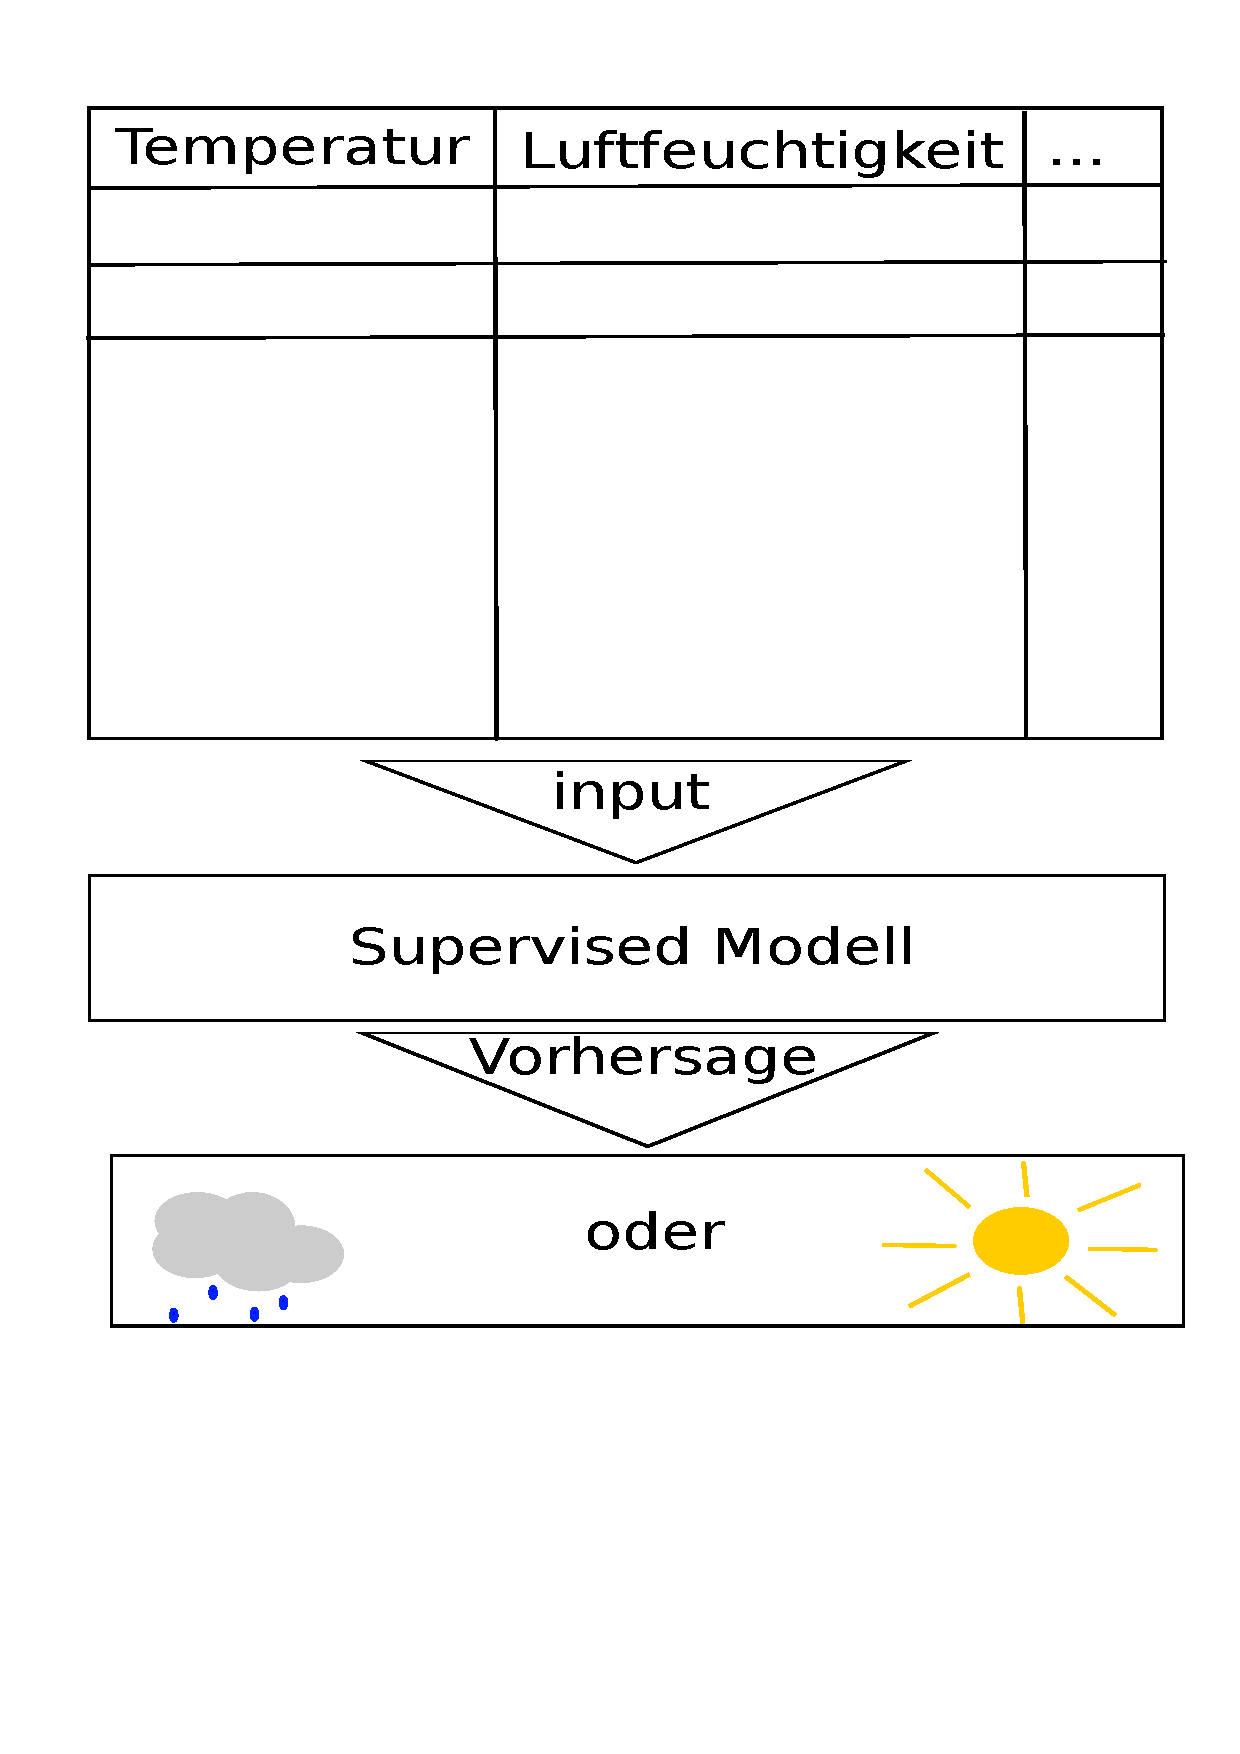
\includegraphics[width=6cm]{Bilder/Label.pdf}
			\caption{Beispiel Wettervorhersage \cite{Sarkar2018}}
			\label{fig:abb1}
		\end{figure}
		
	In der multiklassen Klassifikation können die Inputdaten auf mehr als zwei Klassen aufgeteilt werden, es handelt sich also nicht mehr um eine Ja/Nein-Frage. \cite{Mueller2016} Während der Trainings-Phase werden Regeln für das Zuteilen von Labels erstellt, die später dabei helfen Test-Daten Labels zuzuweisen.  \cite{Suthaharan2016}
	
	\subsubsection{Support Vector Machines}
	Support Vector Maschinen oder auch kurz SVMs, sind vielseitige und mächtige Machine Learning Modelle. Sie zählen zu den beliebtesten Modellen und eignen sich für lineare und nicht-lineare Klassifikation, Regression und zum Erkennen von Anomalien. \cite{Geron2017} SVMs können mathematisch sehr komplex sein und eine hohe Rechenleistung erfordern. \cite{Suthaharan2016} Im Folgenden wird nur die lineare Klassifikation betrachtet.\newline
	Hier ist es möglich zwei Klassen durch eine lineare Trennline eindeutig zu trennen. Diese soll einen Möglichst großen Abstand zu den Datensätzen haben, um später beim Einfügen neuer Daten weniger Fehler zu erzielen.\cite{Geron2017} Da die Trennlinie linear ist, lässt sie sich durch den Term 
		\begin{equation}
		0 = wx^{'} + \gamma
		\end{equation}
	beschreiben. \cite{Suthaharan2016} Der Abstand der Trennlinie zu den beiden nächsten Punkten, die aus verschiedenen Klassen stammen, nennt sich Margin. Die Geraden parallel zur Trennline, durch die zwei Punkte, die diese Grenze bilden, heißen Support Vektoren. In Abbildung \ref{fig:abb10} ist die Trennline die durchgezogene Linie und die Support Vektoren die gestrichelten Linien, der Margin befindet sich zwischen ihnen. Werden während dem Training neue Daten hinzugefügt, die sich außerhalb des Margins befinden, wird das Modell nicht geändert. \cite{Geron2017} Beim Training werden w und $\gamma$ optimiert. \cite{Suthaharan2016}\newline
	
	\begin{figure}[H]
		\centering
		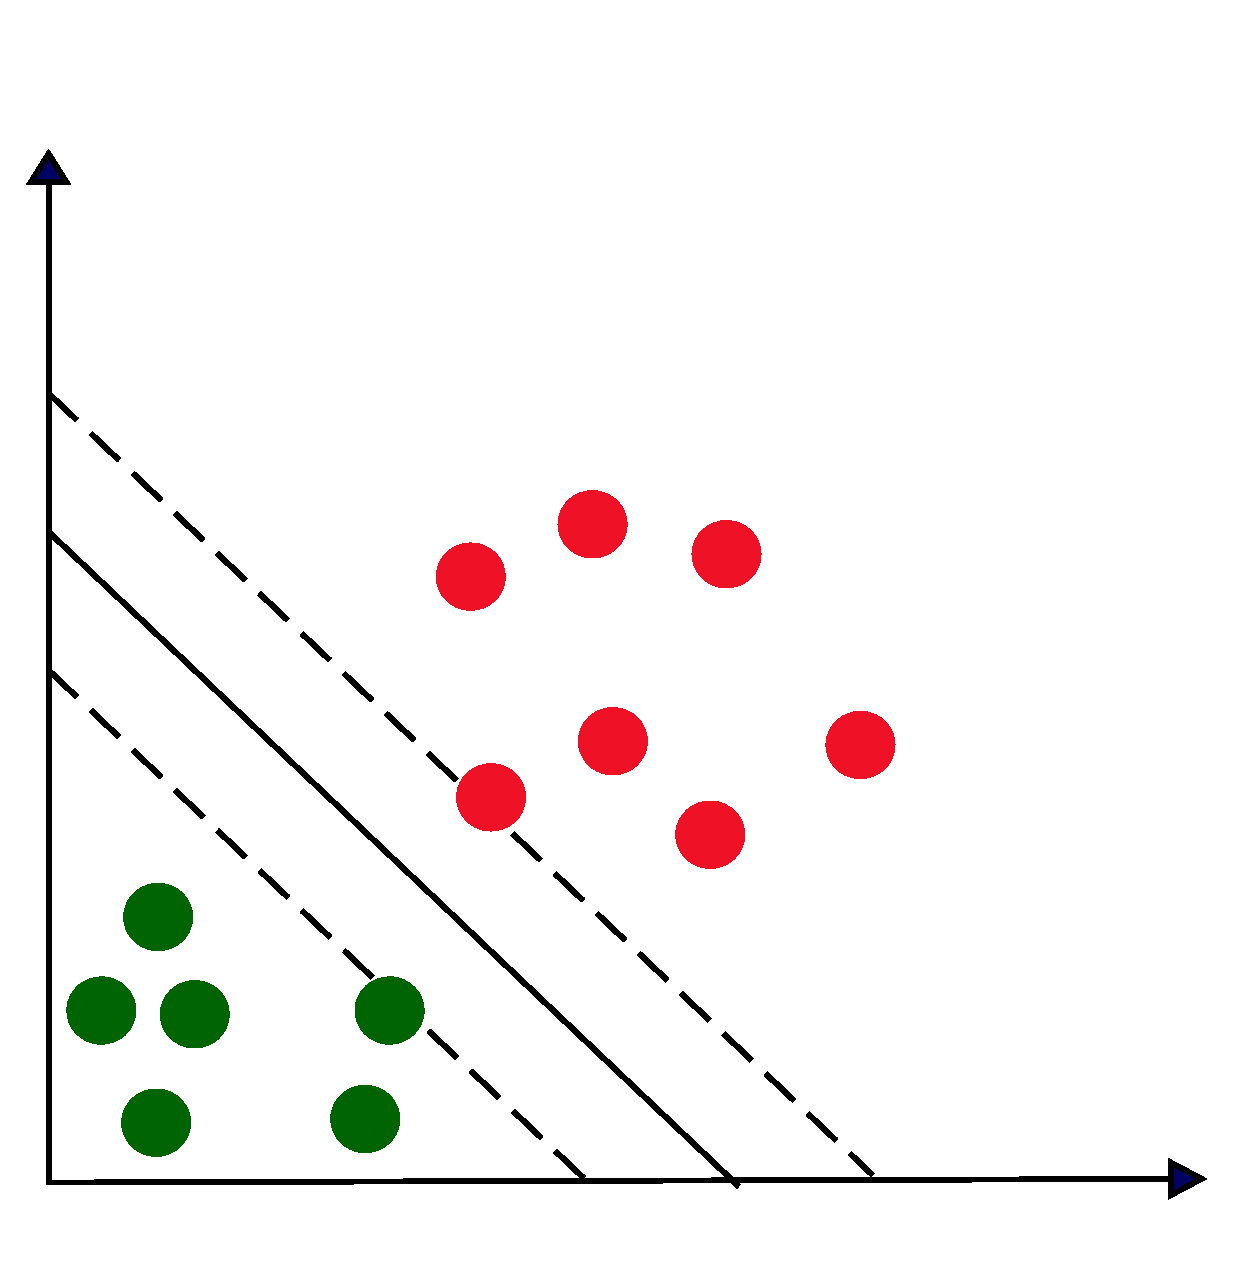
\includegraphics[width=5cm]{Bilder/SVM.pdf}
		\caption{SVM Trennline und Datensätze}
		\label{fig:abb10}
	\end{figure}
	
	Im Folgenden wird mit der scikit-learn Bibliothek ein SVM-Modell erstellt und mit der Funktion fit trainiert. X\_train und y\_train beinhalten die Trainings-Datensätze. Mit Hilfe von predict kann ein neuer Datensatz klassifiziert werden.
	\lstset{style=code}
	\begin{lstlisting}[language=Python]
	def_svc = SVC()
	def_svc.fit(X_train, y_train)
	def_y_pred = def_svc.predict(X_test)
	\end{lstlisting}
	\cite{Sarkar2018}	
	 
	
	\subsection{Regression}
	In Regressions-Problemen sollen oft Zahlen oder Werte ermittelt werden. Im Gegensatz zur Klassifikation gibt es keine Klassen oder Label, denen Daten zugeordnet werden können. Regressions-Modelle lernen stattdessen den Zusammenhang aus Ein- und Ausgangsdaten, um für neue Daten den passenden Output vorherzusagen. \cite{Sarkar2018}
	 \newline
	Abbildung \ref{fig:abb2} zeigt ein Beispiel bei dem mit Hilfe von Datensätzen, die Informationen zu Eiskäufen pro Minute und der Temperatur enthalten, eine Funktion gelernt werden konnte, um für zukünftige Temperaturen die passende Anzahl an Eiskäufen pro Minute auszugeben. \cite{Sarkar2018}
	\newline
	
	\begin{figure}[H]
		\centering
		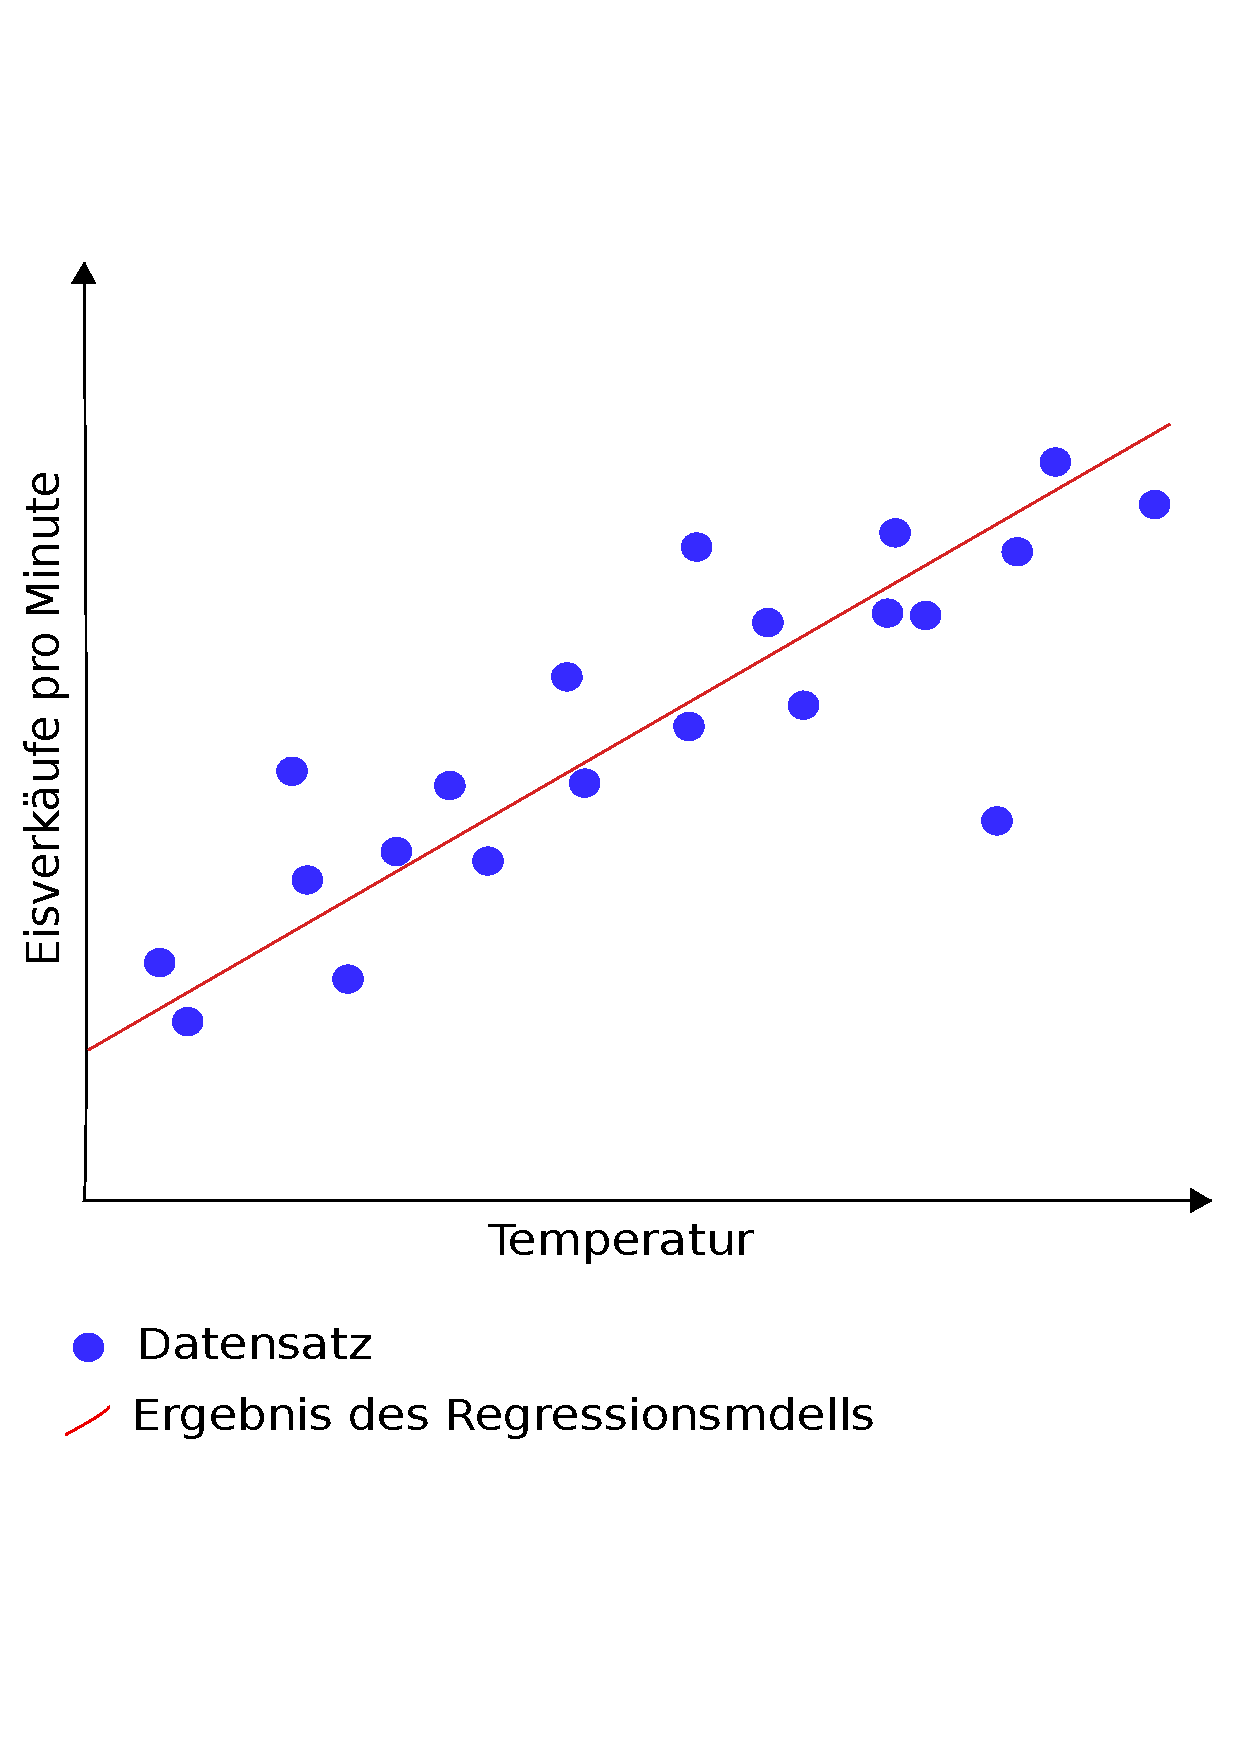
\includegraphics[width=5cm]{Bilder/Regression.pdf}
		\caption{Beispiel Regression}
		\label{fig:abb2}
	\end{figure}
	
	Lineare Regressions Modelle versuchen mit nur einer Variable x eine Output-Variable y zu bestimmen und können somit lineare Probleme lösen. \cite{Sarkar2018}
	\newline
	Multivariable Regressions Methoden werden für Probleme mit mehreren input-Variablen in Form eines Vektors und nur einer output-Variable verwendet. \cite{Sarkar2018}
	 \newline
	Ein Sonderfall der Multivariablen Regression ist die Polynomiale Regression. Hier ist die Ausgabevariable Polynom n-ten Grades der Eingangsvariable. \cite{Sarkar2018}
	\newline
	Nichtlineare Regressions Modelle stellen zwischen ein- und ausgehenden Daten eine Beziehung auf Basis einer Kombination aus nicht-linearen Funktionen her. \cite{Sarkar2018}
	\newline
	%Lasso regression is a special form of regression that performs normal regression and generalizes the
	%model well by performing regularization as well as feature or variable selection. Lasso stands for least absolute
	%shrinkage and selection operator. The L1 norm is typically used as the regularization term in lasso regression
	%Ridge regression is another special form of regression that performs normal regression and generalizes
	%the model by performing regularization to prevent overfitting the model. Typically the L2 norm is used as the
	%regularization term in ridge regression 
	%Generalized linear models are generic frameworks that can be used to model data predicting different
	%types of output responses, including continuous, discrete, and ordinal data. Algorithms like logistic
	%regression are used for categorical data and ordered probit regression for ordinal data.(Sarkar, S.38)
	
	
	\newpage
	
	\section{Unsupervised Learning}
	 Bei Unsupervised Learning haben die Trainings-Daten keine Label. \cite{Sarkar2018} Es ist also kein erwarteter Output bekannt und auch schwer feststellbar ob das Modell korrekte Ergebnisse erzielt. Der Algorithmus bekommt nur die Input-Daten. Er muss anhand dieser Entscheidungen treffen und kategorisieren. \cite{Mueller2016}\newline
	 Das Modell lernt inherente Strukturen, Muster und Beziehungen aus dem Datensatz, ohne dabei Hilfe von außen zu bekommen. \cite{Sarkar2018} Hierbei werden besondere Auffälligkeiten im Datensatz gefunden. \cite{Kirk2014} Die Ergebnisse sind unsicherer als die von Supervised Learning Algorithmen. Sie eignen sich aber, um weitere Informationen zu den Daten zu finden. \cite{Sarkar2018} Deshalb wird diese Art des Machine Learnings oft in explorativen Bereichen eingesetzt, um Daten besser zu verstehen. Unsupervised Learning kann als Vorverarbeitungsschritt des Supervised Learnings eingesetzt werden. Hierbei sollen neue Representatoren für die Daten gefunden werden, um Genauigkeit, Speichernutzung und Geschwindigkeit zu verbessern. \cite{Mueller2016}
	 Unsupervised Learning kann durch verschiedene Methoden angewendet werden: Clusterbildung, Dimensionsreduktion, Anomalie Erkennung und Association rule-mining. \cite{Sarkar2018} Diese werden im Folgenden behandelt.
	 
	 \subsection{Clusterbildung}
	 Ziel der Clusterbildung ist es, dass sich in einem Cluster möglichst ähnliche Daten befinden, die sich zu den Daten außerhalb des Clusters unterscheiden. \cite{Mueller2016} Die Cluster werden durch Muster, Ähnlichkeiten und Verbindungen zwischen den Datensätzen gebildet. \cite{Sarkar2018} Zum Beispiel werden die Elemente in Abbildung \ref{fig:abb3} nach Formen in die Cluster rot, grün und blau eingeordnet. \cite{Sarkar2018}
	  %Die Clusterbildung kann in verschiedene Typen aufgeteilt werden: Centroid based, Hirachical clustering, distribution based und density based. \cite{Sarkar2018}
	 \begin{figure}[h!]
	 	\centering
	 	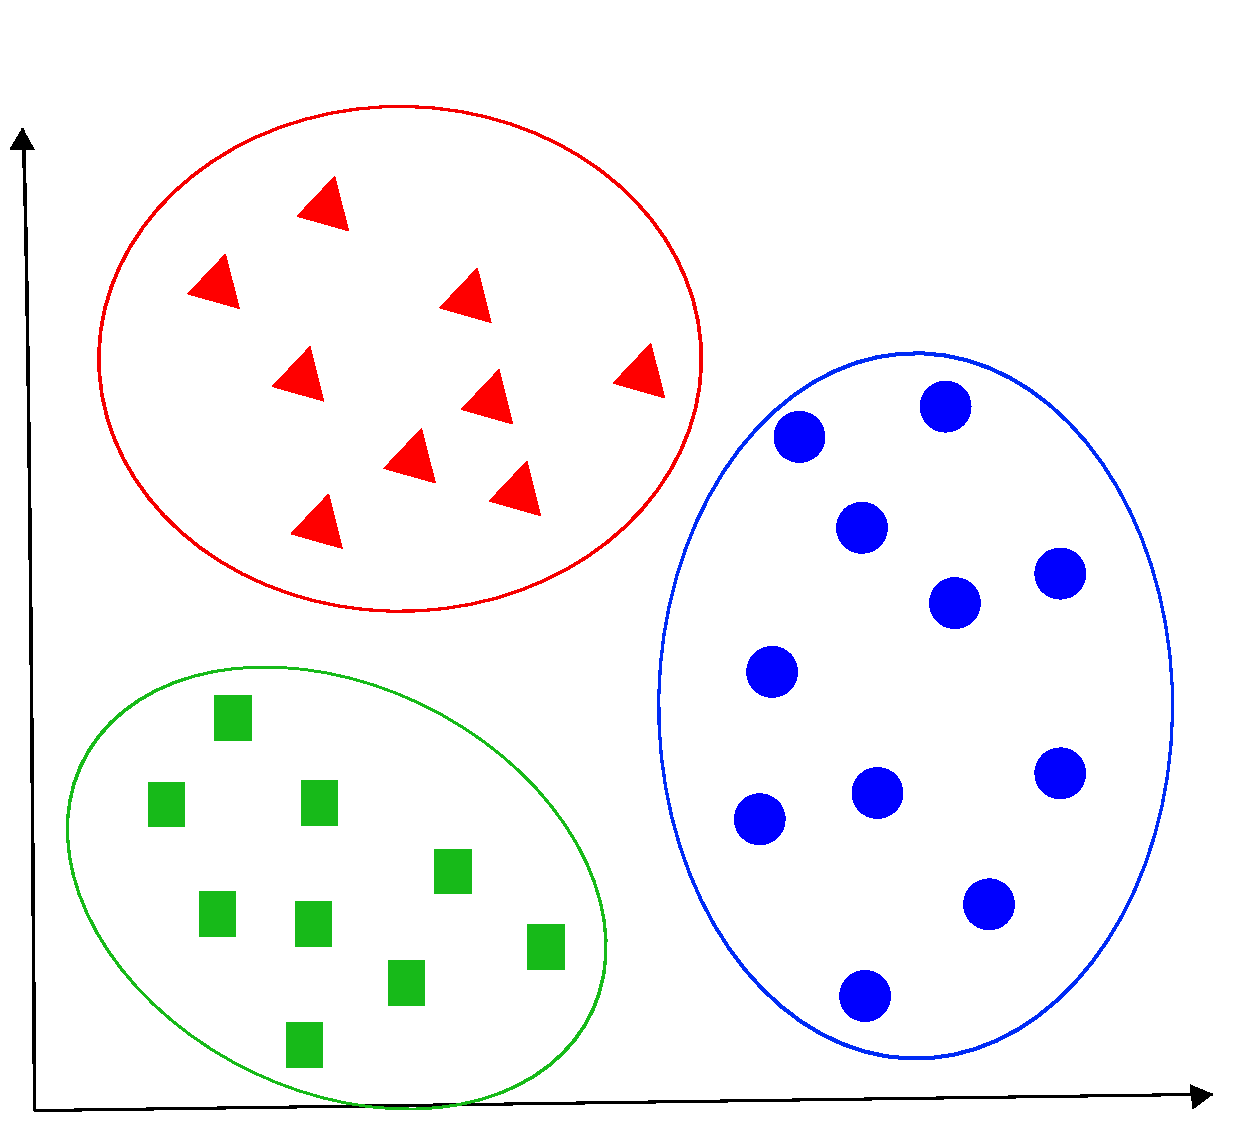
\includegraphics[width=5cm]{Bilder/Cluster.pdf}
	 	\caption{Cluster}
	 	\label{fig:abb3}
	 \end{figure}
	 
	 	\subsubsection{K-Means Algorithmus}
	 	Der K-Means Algorithmus verwendet die Clusterbildung. K steht hierbei für die Anzahl der Cluster, die gebildet werden sollen. \cite{Kirk2014} Es wird versucht, einen Mittelpunkt in jedem Cluster zu finden. Dieser ist der Punkt, der den geringsten Abstand zu allen anderen Punkten in der Region hat. \cite{Mueller2016} Vorteile dieses Algorithmus sind, dass die Cluster sehr genau und kugelförmig sind und der Algorithmus sich einer Lösung annähert. \cite{Kirk2014} \newline
	 	Zu Beginn werden K zufällige Punkte aus dem Datensatz ausgewählt und als Mittelpunkt verwendet. \cite{Kirk2014} Danach werden die verbleibenden Datensätze dem Mittelpunkt mit dem geringsten Abstand zugeordnet und neue Mittelpunkte bestimmt. Diese haben den jeweils geringsten Abstand zu allen anderen Punkten im Cluster. Es werden so lange neue Mittelpunkte bestimmt und Punkte zu neue Clustern zugeordnet, bis es keine Veränderung mehr gibt. \cite{Mueller2016} Der Abstand der Punkte kann mit verschiedenen Methoden berechnet werden. Eine davon ist die Euklidische Distanz, siehe Formel (2). \cite{Kirk2014}
	 	\begin{equation}
	 	d_{euklid}(x,y)= \sqrt{\sum_{i=1}^{n}(x_i - y_i)^2}
	 	\end{equation}
	 	
	 	Im Folgenden wird Beispiel-Code für den Algorithmus erklärt und gezeigt. Hierzu wir die Programmiersprache Python verwendet. Es handelt sich hierbei nur um einen Codeauszug und nicht um ein ganzes Programm.
	 	
	 	\begin{lstlisting}[language=Python]
	 		kmeans = KMeans(n_clusters = 3)
	 		kmeans.fit(X)
	 	\end{lstlisting}
	 	In diesem Abschnitt wird ein K-Means Modell erzeugt und mit Hilfe der Funktion fit trainiert. X enthält die zweidimensionalen Datensätze. Das Modell und die Funktion werden bereits von der scikit-learn Bibliothek bereitgestellt.
	 		\begin{lstlisting}[language=Python]
	 		kmeans.predict(Z)
	 		\end{lstlisting}
	 	Mit predict können nach dem Training den Clustern neue Datensätze Y zugeordnet werden. Die Mittelpunkte und damit auch die Cluster werden dabei nicht mehr verändert. \cite{Mueller2016}
	 	
	 
	 
	 \subsection{Dimensionsreduktion}
	 Die Komplexität des Machine Learning Modells ist abhängig von der Anzahl der Inputs. Sie bestimmen die Zeit- und Speicherkomplexität, sowie die Anzahl der zum Training benötigten Daten. \cite{Alpaydin2004} Dimensionsreduktion wird genutzt um den überladenen Input-Space zu verkleinern. Somit wird die Anzahl der relevanten Features oder Attribute($\widehat{=}$ Dimensionen) für jeden Datensatz reduziert. \cite{Sarkar2018} Wenn die Modelle einfach gehalten werden, sind sie, aufgrund ihrer geringeren Varianz, bei kleinen Datensätzen robuster. \cite{Alpaydin2004} Die Reduktion der Dimensionen erfolgt durch die Auswahl von Hauptfeatures und bedarfsgesteuerten Features. Für diese gibt es zwei Methoden. \cite{Sarkar2018}
	 \newline
	 Für die Feature Extraction werden neue Features, die Kombinationen aus der origninalen Featureliste sind, gesucht. \cite{Alpaydin2004}
	 \newline
	 Bei der Feature Selection werden von d Dimensionen k, mit Hilfe von Subset Selection, ausgewählt. \cite{Alpaydin2004} Die Features, die die meisten Informationen liefern, werden aus der originalen Featureliste ausgewählt, der Rest wird verworfen. Es kommen keine neuen Features hinzu. \cite{Sarkar2018}\newline
	 Ziel der Subset Selection ist es, das beste Subset aus der Featureliste mit einer möglichst geringen Anzahl von Dimensionen und der besten Genauigkeit zu finden. Es gibt $2^{d}$ mögliche Subsets aus denen ausgewählt werden kann. Aufgrund der großen Menge können nicht alle getestet werden, deswegen müssen geeignete Verfahren für die Auswahl genutzt werden. \cite{Alpaydin2004}
	 
	 \subsection{Anomalie Erkennung}
	 Ziel der Anomalie Erkennung ist es, seltene oder laut vorherigen Datensätzen untypische Ereignisse zu erkennen, wie in Abbildung. \ref{fig:abb4} Hier fällt auf, dass ein Wert stark von den Anderen abweicht. \newline
	 Anomalien können auch nach bestimmten Mustern auftreten. In der Trainings-Phase haben alle Input-Daten keine Anomalien, um später Abweichungen von der Norm zu erkennen. Danach kann der Algorithmus zwischen normalen und anomalen Datensätzen unterscheiden. \cite{Sarkar2018}
	 \begin{figure}[h!]
	 	\centering
	 	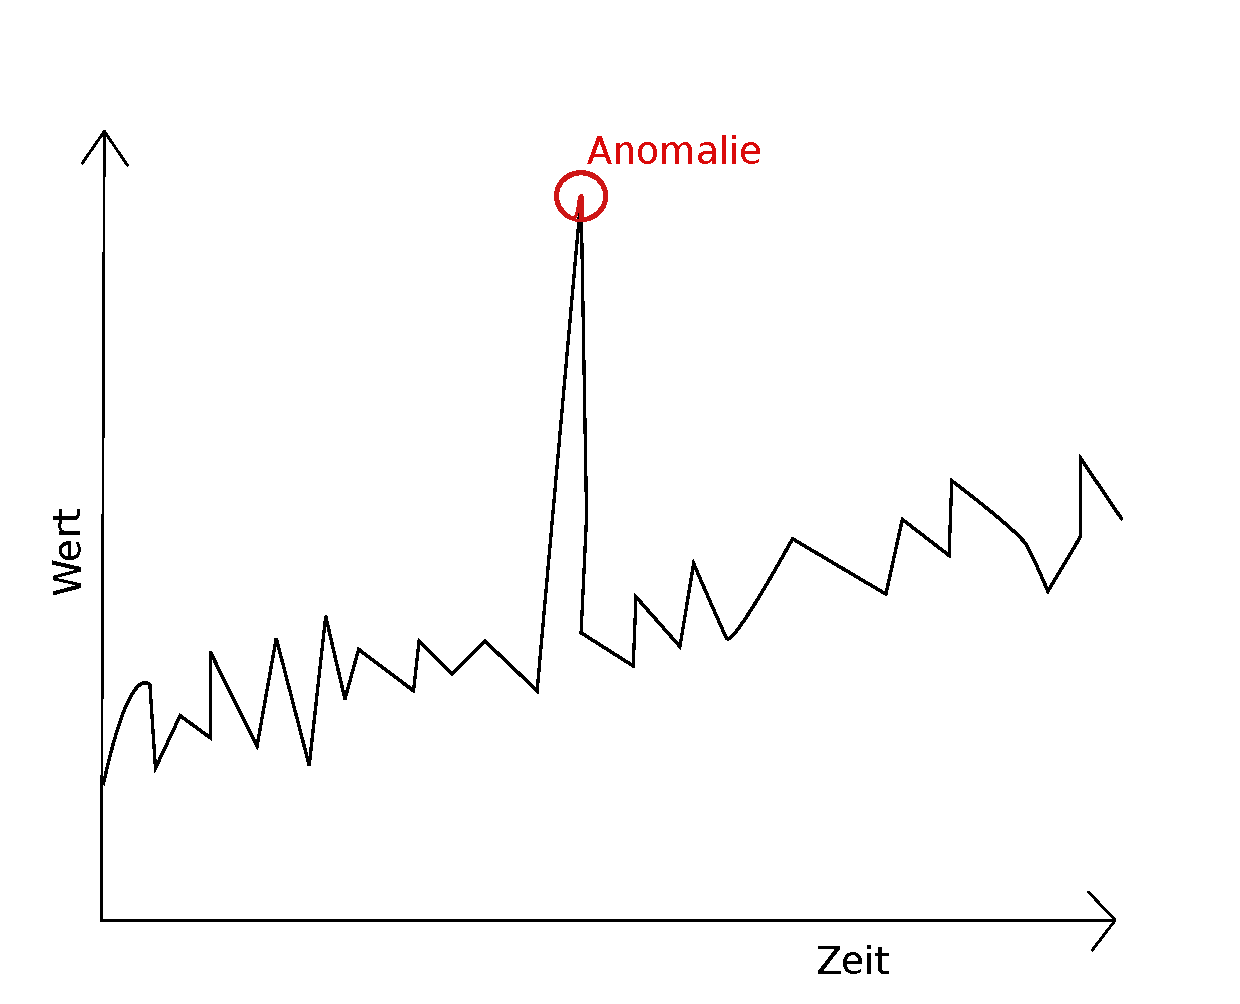
\includegraphics[width=5cm]{Bilder/Anomalie.pdf}
	 	\caption{Anomalie}
	 	\label{fig:abb4}
	 \end{figure}
	 
	 \subsection{Association rule-mining}
	 Beim Association rule-mining werden Transaktionsdaten untersucht und analysiert, um Muster, sowie mögliche Regeln zu bestimmen. Diese Methode wird auch "market basket analysis" genannt, da sie oft genutzt wird um Einkaufsmuster zu erkennen. \cite{Sarkar2018} \newline
	 In Abbildung \ref{fig:abb5} werden die verschiedenen Formen mit Association rule-mining analysiert. Das Ergebnis ist, dass der Kreis und das Quadrat häufig zusammen auftreten. Als neue Regel kann also zum Beispiel festgehalten werden, dass es sehr wahrscheinlich ist, dass sich ein Quadrat in einem Bereich befindet, wenn sich dort auch ein Kreis befindet. \newline
	 Anhand von Ergebnissen dieser Art können zum Beispiel Produktvorschläge basierend auf dem eigenen Warenkorb und den Käufen anderer Nutzer gemacht werden.
	\begin{figure}[H]
		\centering
		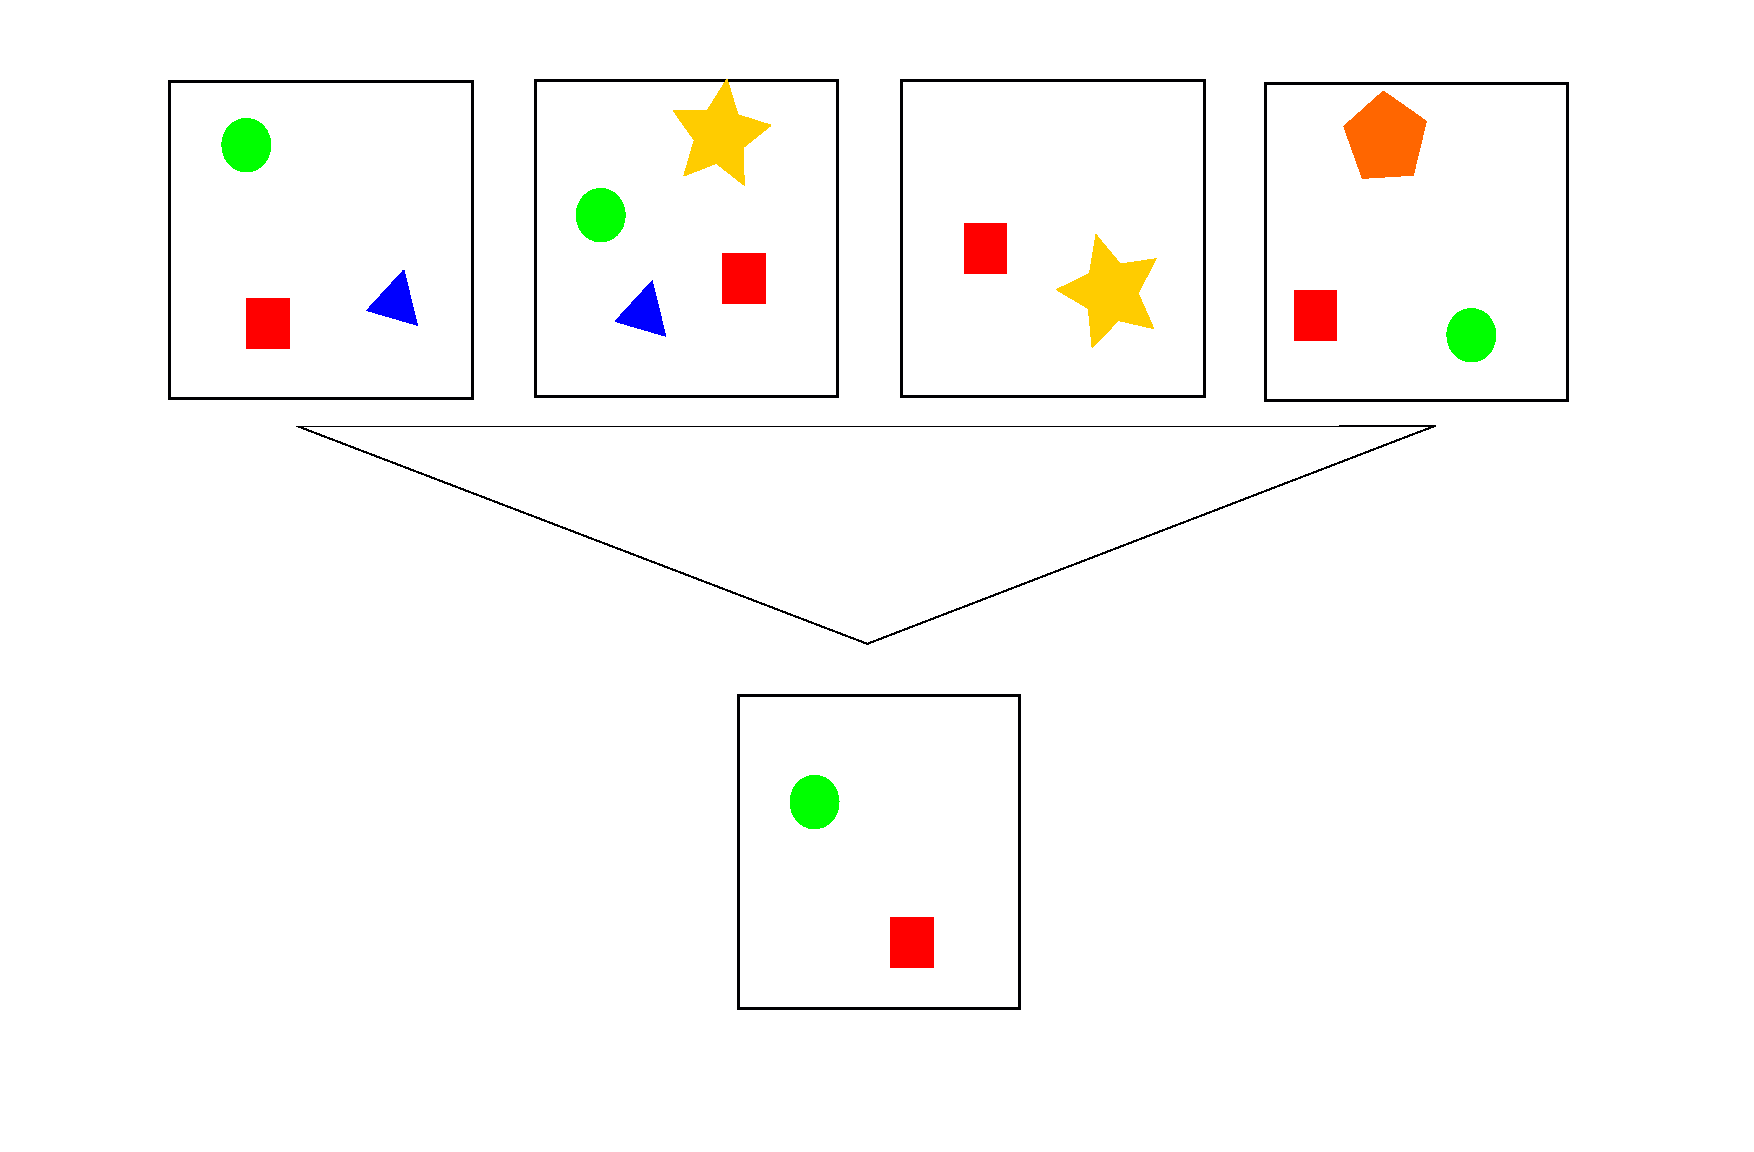
\includegraphics[width=5cm]{Bilder/rule-mining.pdf}
		\caption{Association rule-mining}
		\label{fig:abb5}
	\end{figure}
	\newpage
	
	\section{Reinforcement Learning}
	Beim Reinforcement Learning setzt man intelligente Programme, welche auch Agenten genannt werden, ein. Hierbei gibt es keine Trainings-Daten. \cite{Nandy2018} Ein Agent trainiert um sich seiner Umgebung anzupassen und seine Leistung zu verbessern. \cite{Sarkar2018} \newline
	Er kennt den Zustand, in dem sich seine Umgebung befindet und führt Aktionen aus, um diesen zu verändern. Das Ausführen von Aktionen von einem Start- bis zu einem Endzustand nennt man Episode oder Prozess. \cite{Alpaydin2004}\newline  
	Die Umgebung kann eine 2D oder 3D Simulation eines Szenarios aus der echten Welt oder aus einem Spiel sein.  
	Die Wahl der Aktionen erfolgt durch Ausprobieren, da es sehr schwer ist von Beginn an vorauszusagen, welche Aktion in welchem Zustand ausgeführt werden muss. \cite{Nandy2018} Der Agent besitzt bereits zu Beginn bestimmte Strategien und Richtlinien, welche verbessert und angepasst werden. \cite{Sarkar2018}
	Abhängig von der Interaktion mit der Umgebung erhält der Agent von der Umgebung Belohnungen und Bestrafungen, meist in Form von plus und minus Punkten. \cite{Nandy2018} Diese führen zu einem Update der Strategien, um später mehr Belohnungen zu erhalten. \cite{Sarkar2018}\newline
	\begin{figure}[H]
		\centering
		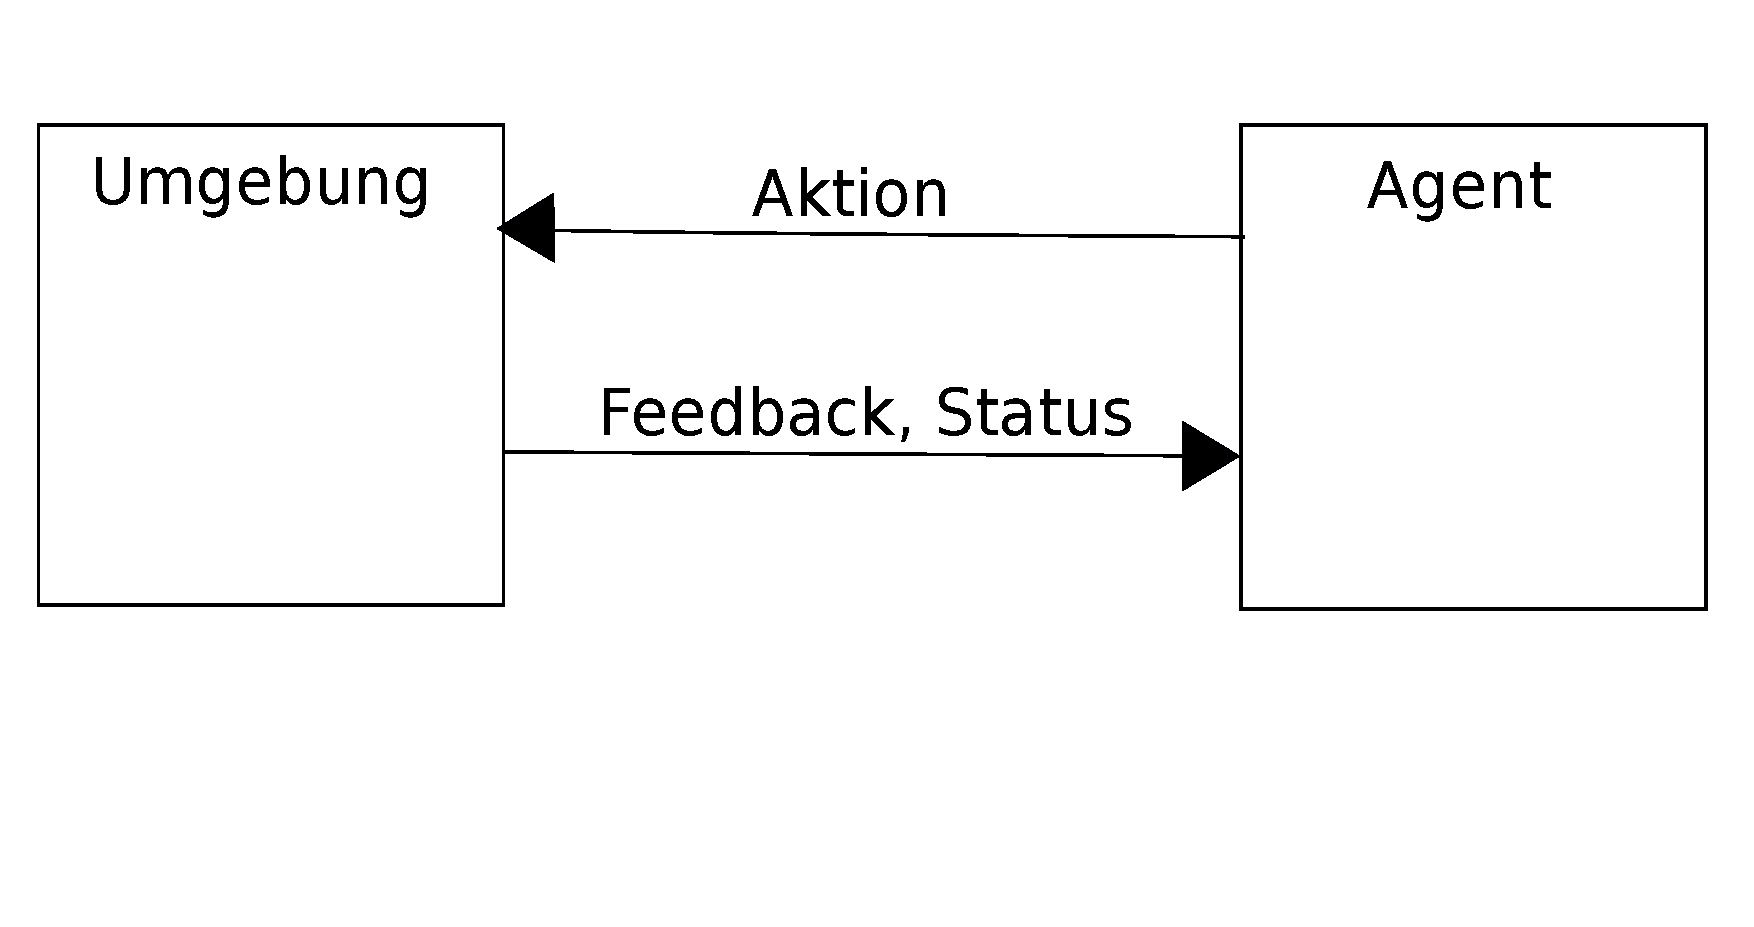
\includegraphics[width=5cm]{Bilder/Reinforcement.pdf}
		\caption{Umgebung mit Agent}
		\label{fig:abb6}
	\end{figure}
	Reinforcement Learning wird auch Lernen mit einem Kritiker genannt, da dem Modell im Lernprozess nicht vorgegeben wird was es tun soll. Erst nach dem Ausführen der Aktionen, wird eine Rückmeldung über diese an das Modell weitergegeben. \cite{Alpaydin2004}
	
	\subsection{Umgebung}
	Die Umgebung des Agenten kann mit bestimmten Eigenschaften beschrieben werden, diese werden im Folgenden erläutert. \cite{Nandy2018} \newline
	Ist die Umgebung deterministisch gibt es für jede Aktion nur einen Übergang zu einem anderen Zustand. Ist sie nicht-deterministisch sind mehrere Übergänge für jede Aktion möglich. \cite{Nandy2018}\newline
	Ist die Umgebung beobachtbar, können wie bei einem Schachspiel, alle Informationen über die Umgebung wahrgenommen werden. Wenn die Umgebung nur teilweise beobachtbar ist, sind bestimmte Informationen versteckt, wie zum Besipiel beim Poker die Handkarten der anderen Mitspieler. \cite{Nandy2018}\newline
	Eine Umgebung ist fortlaufend, wenn es mehr als eine Aktion gibt, um zum nächsten Zustand zu gelangen. Ist sie beschränkt, gibt es nur eine Aktion, die zum nächsten Zustand führt. \cite{Nandy2018}
	\begin{figure}[h!]
		\centering
		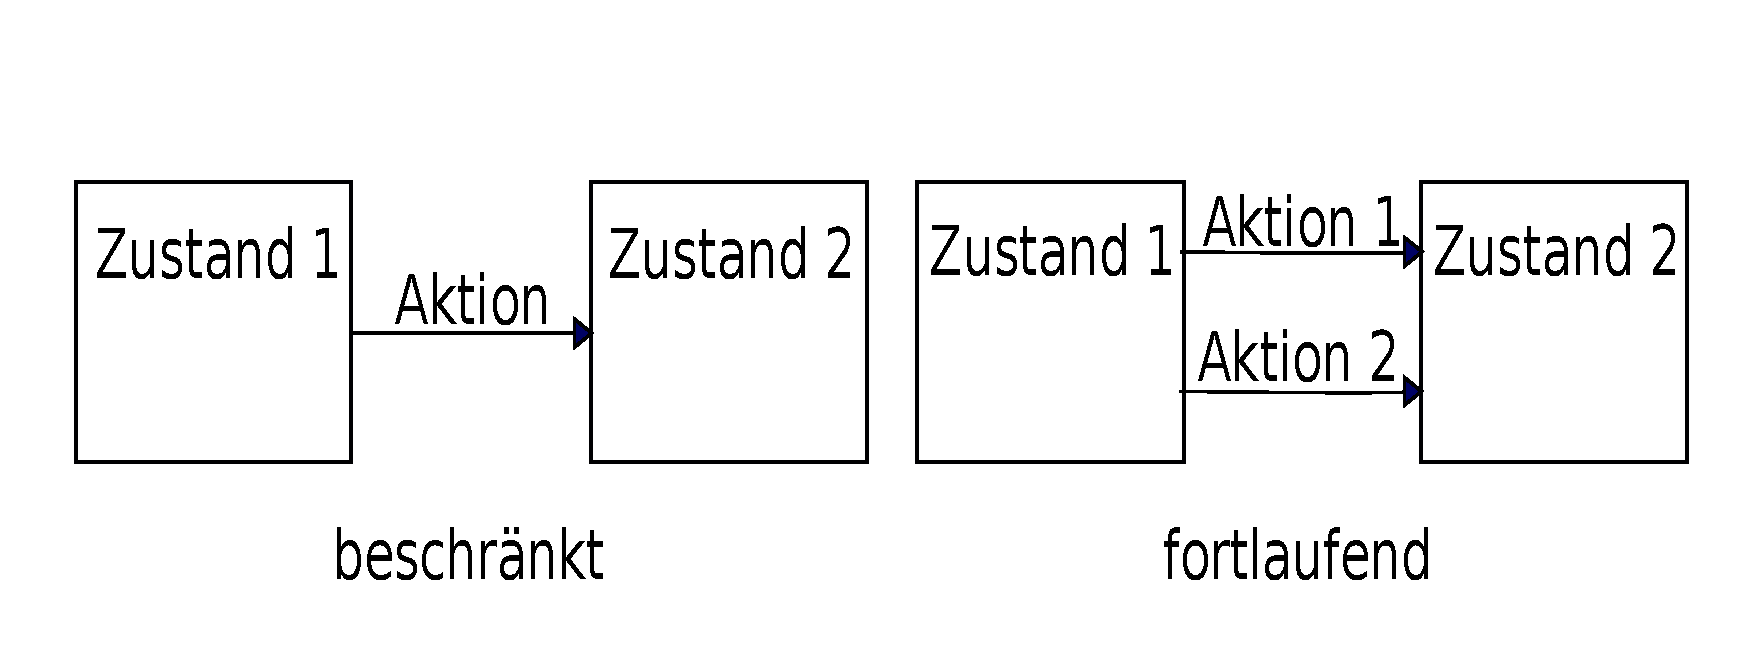
\includegraphics[width=8cm]{Bilder/Umgebung.pdf}
		\caption{beschränkte und fortlaufende Umgebung}
		\label{fig:abb7}
	\end{figure} \newline
	Es gibt multi-agent Umgebungen, die für Problemstellungen mit mehrere Umgebungen, verschiedenen Aufgaben und ähnlichen Entscheidungen geeignet sind. Hier gibt es oft mehr als eine Aktion, um zum nächsten Status zu gelangen. Dies wird durch Kommunikation zwischen den Agenten ermöglicht. Die Umgebung kann bei einer multi-agent Problemstellung dynamisch sein, was bedeutet, dass es Veränderungen der Umgebung an Interaktionsstellen geben kann. In single-agent Umgebungen gibt es nur eine Umgebung, da keine Kommunikation zwischen Agenten möglich ist. \cite{Nandy2018}
	\begin{figure}[H]
		\centering
		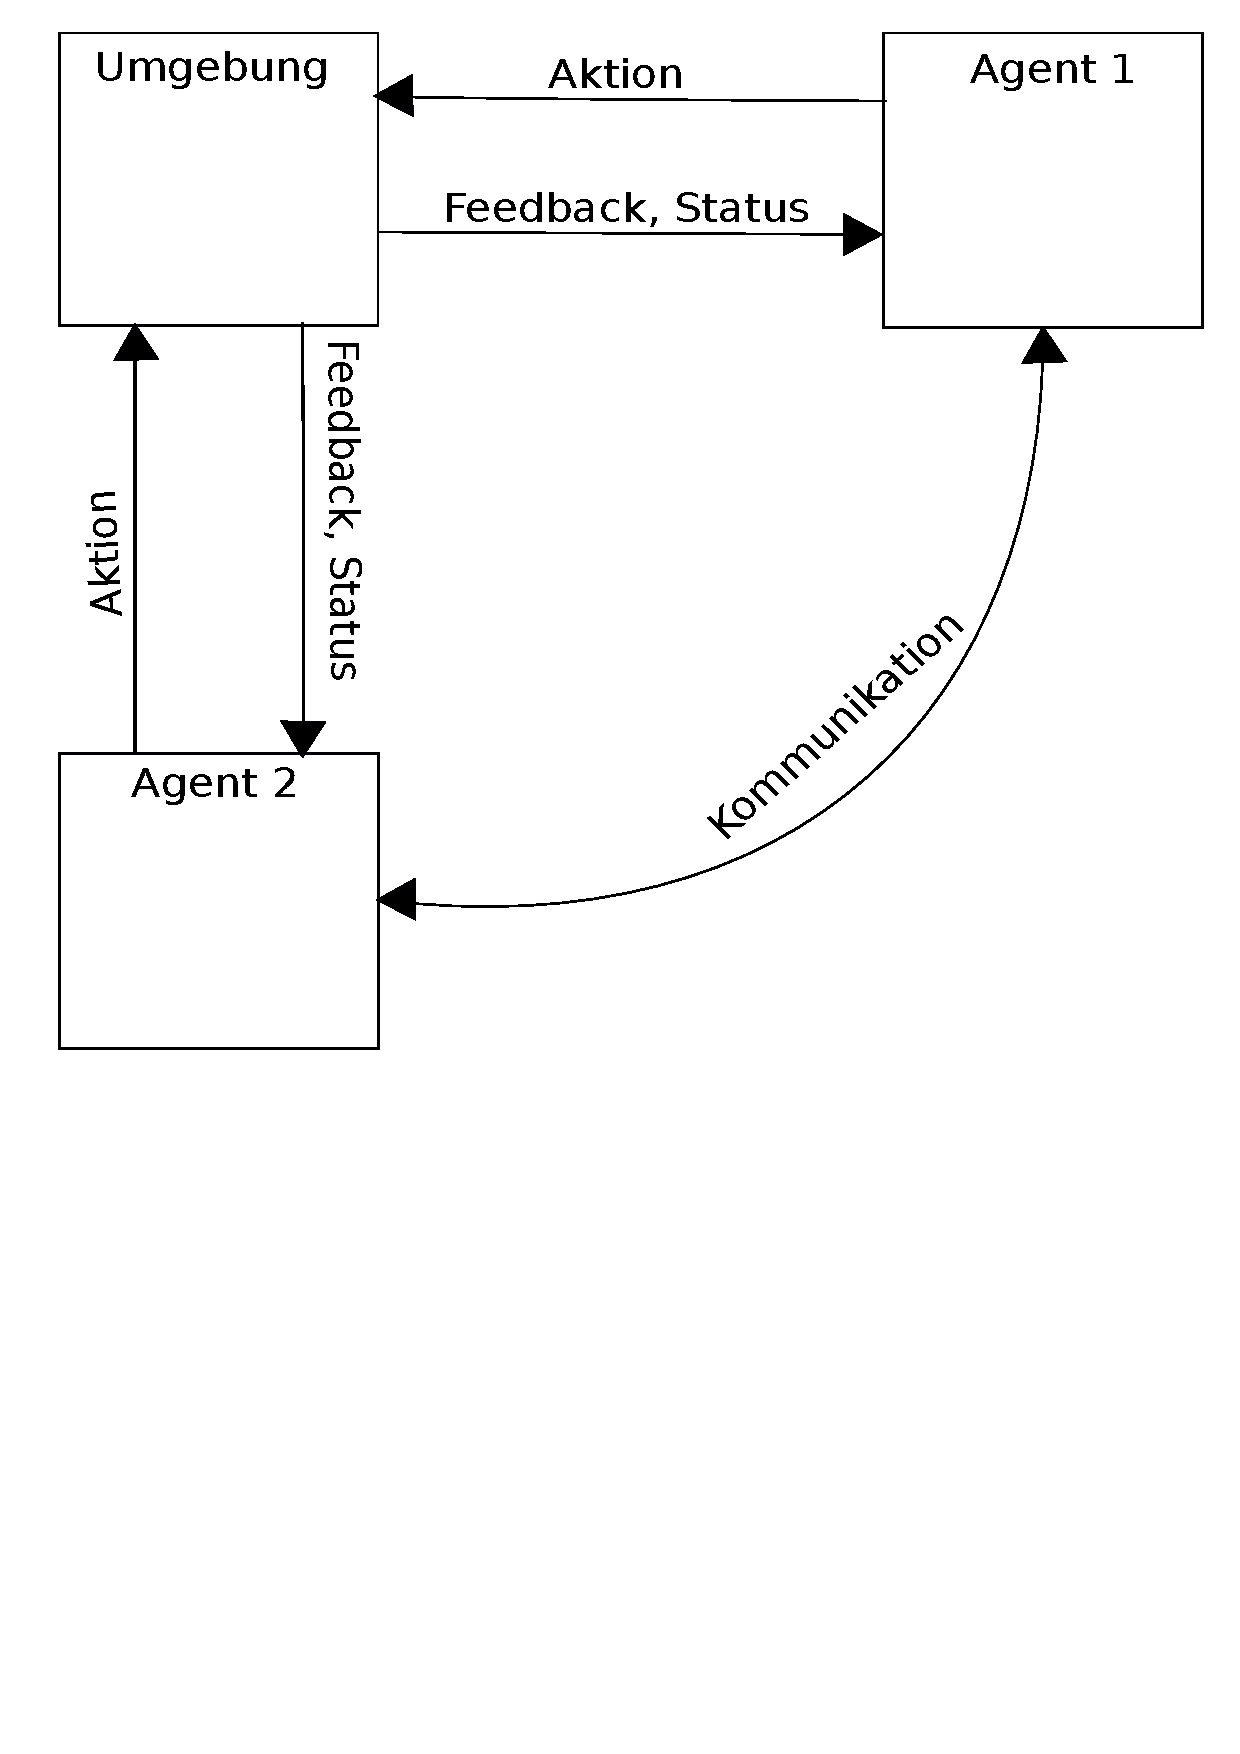
\includegraphics[width=5cm]{Bilder/multiagent.pdf}
		\caption{Umgebung mit zwei Agenten}
		\label{fig:abb8}
	\end{figure}

	\subsection{Einsatzbereiche}	
	Reinforcement Learning wird in der Produktion von Robotern genutzt, um Objekte von einer Box in eine andere zu befördern. In der Lagerverwaltung werden Transportzeiten zwischen Lagern verringert und die Platznutzung im Lager durch Reinforcement Learning optimiert. Die Fahrzeugnutzung in der Lieferverwaltung kann damit ebenfalls optimiert werden. Im Finanzbereich wird unter Verwendung von Handelsstrategien die Buchhaltung unterstützt. \cite{Nandy2018}
	
	\newpage
	
	\section{Fazit}
		Abschließend lässt sich sagen, dass die drei Machine Learning Arten sehr unterschiedliche Nutzen haben.
	Supervised Learning eignet sich zur Zuordnung von Daten in bestimmte Kategorien und zur Abschätzung von Funktionen aus Datensätzen und damit zum Voraussagen von Ergebnissen für neue Werte. Beim Unsupervised Learning gibt es oft keine eindeutigen oder sofort zu Problemlösung verwertbaren Ergebnisse. Diese Art des Machine Learnings eignet sich zu Unterstützung von Supervised Algorithmen. Reinforcement Learning unterscheidet sich drastisch von den anderen Methoden. Hier werden nicht aus Datenmengen Informationen gesammelt, sondern durch Belohnungen Verhaltensmuster optimiert. Diese Vorgehensweise ermöglicht völlig andere Problemstellungen als bei Supervised und Unspuervised Learning. Aufgrund der Vielfalt der Machine Learning Arten sind alle sehr bedeutend, da sie auf sich stark unterscheidende Problemstellungen angewandt werden können.
	
	\newpage
	
	\printbibliography
	
\end{document}